%%%%%%%%%%%%%%%%%%%%%%%%%%%%%%%%%%%%%%%%%%%%%%%%%%%%%%%%%%%%%%%%%%%%%%%%%%%%%%%%%%%%%%%%%
% Section 8: Importing RSCPs and exporting TCPs
%	This section contains a description of the following:
%	- The contents of RapidSmith Checkpoints (RSCP)
% 	- How to load a RSCP into RapidSmith2 
%	- The contents of Tincr Checkpoints (TCP)
% 	- How to export a TCP from RapidSmith2 
%	- Important information that is imported from RSCP and how they are
% 		represented in RapidSmith2 (such as routethroughs) 	
%	- Code samples for importing RSCPs and exporting TCPs
%%%%%%%%%%%%%%%%%%%%%%%%%%%%%%%%%%%%%%%%%%%%%%%%%%%%%%%%%%%%%%%%%%%%%%%%%%%%%%%%%%%%%%%%%
\newpage

\section{Design Import/Export} \label{sec:import}
\graphicspath{{./techReportFigures/sec8_importExport/}{./techReportFigures/sec2_background/}}

RapidSmith2 supports modifiying Vivado designs post-synthesis, post-place, and
post-route as shown in \autoref{fig:rs2Flow}. As the figure shows, RapidSmith
Checkpoints (RSCP) are generated from \texttt{Tincr} which are parsed and loaded
into RapidSmith2 \texttt{CellDesign} data structures. After a CAD tool has been
run, a RapidSmith2 \texttt{CellDesign} can be converted to a Tincr Checkpoint
(TCP), which can then be loaded back into Vivado to complete the remainder of
the implementation flow. This section details how to load a RSCP into
RapidSmith2, and generate TCP from a \texttt{CellDesign}.

\begin{figure}[htb]
\centering
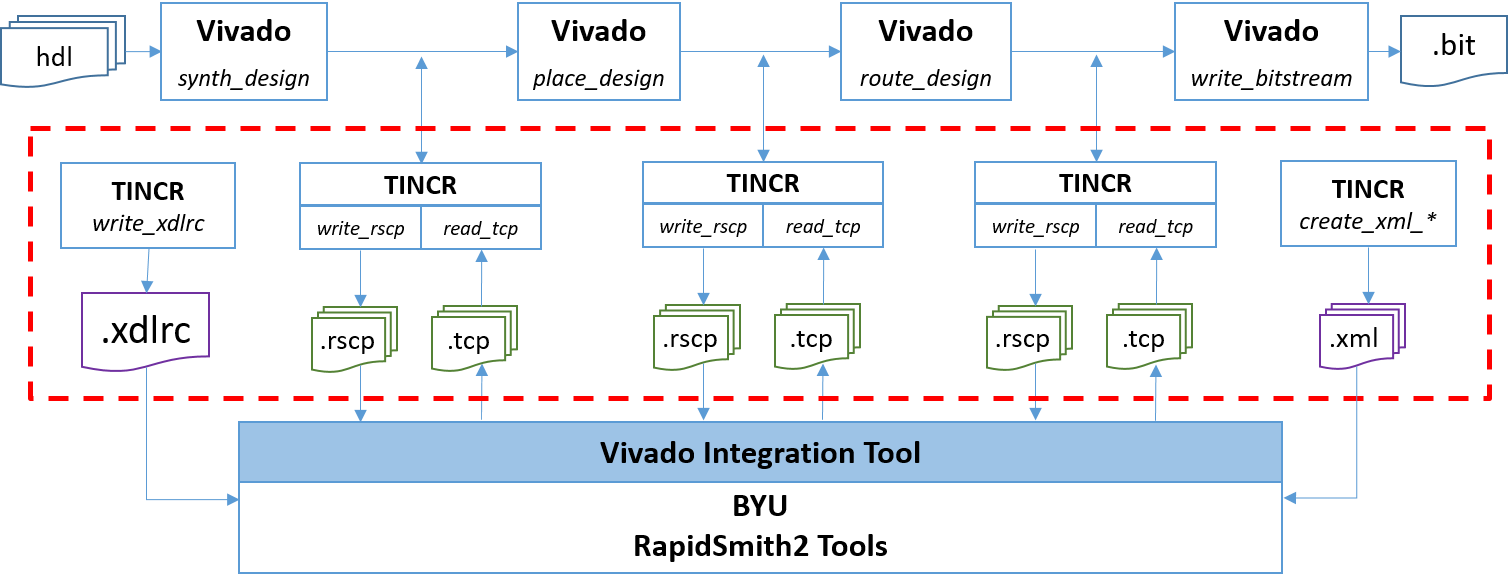
\includegraphics[width=\columnwidth]{usageModel.png}
\caption{RapidSmith2 Design Flows}
\label{fig:rs2Flow}
\end{figure}

After a Vivado design has been converted to a RSCP using the \texttt{Tincr}
command \texttt{[::tincr\-::write\_rscp]} , the RSCP can be loaded into
RapidSmith2 using the code shown on lines 2-5 in \autoref{code:import}.

\begin{lstlisting}[xleftmargin=1.5em, framexleftmargin=1.5em, caption=How to
import RSCP and export TCP files to and from RapidSmith2, label=code:import]
  // Loading a RapidSmith Checkpoint
  VivadoCheckpoint vcp = VivadoInterface.loadRSCP("pathToCheckpoint.rscp");
  CellDesign design = vcp.getDesign();
  Device device = vcp.getDevice();
  CellLibrary libCells = vcp.getLibCells();

  // Insert CAD Tool Here

  // Exporting the modified design to a Tincr Checkpoint
  VivadoInterface.writeTCP("pathToStore.tcp", design, device, libCells);
\end{lstlisting}

\vspace{.3cm}
\noindent
While a design is being imported into RapidSmith2, several useful additional
data structures are built up. To gain access to those data structures, you can pass
an additional argument into the \texttt{VivadoInterface::loadRSCP()}, as shown
in \autoref{code:import2}.

\begin{lstlisting}[xleftmargin=1.5em, framexleftmargin=1.5em, caption=Importing
a RSCP with additional information, label=code:import2]
  // Loading a Tincr Checkpoint with additional info
  VivadoCheckpoint vcp = VivadoInterface.loadRSCP("PathToCheckpoint.rscp", true); 
  Collection<BelRoutethrough> belRts = vcp.getRoutethroughObjects();
  Collection<Bel> staticSources = vcp.getStaticSourceBels();
  Map<BelPin, CellPin> belPinToCellPinMap = vcp.getBelPinToCellPinMap()
\end{lstlisting}

\vspace{.3cm}
\noindent
Line 10 of \autoref{code:import} demonstrates how to export a design from
RapidSmith2, which produces a Tincr Checkpoint (TCP). To import the TCP back
into Vivado, simply open Vivado in Tcl mode and run the command
\texttt{[tincr::read\-\_tcp myCheckpoint.tcp]}

\subsection{Import Notes}
There are a few things to be aware of when a design is converted from a RSCP to
a RapidSmith2 \texttt{CellDesign}. 

\begin{itemize}
  \item All VCC nets of the RSCP are combined into a single VCC net while
  translating the EDIF to a \texttt{Cell\-Design}. The same applies for GND
  nets.
  The API calls \texttt{CellDesign::get\-VccNet()} and
  \texttt{CellDesign::get\-GndNet()} can be used to obtain a handle to each
  static net in the design.
  
  \item The used site PIPs of each site are parsed and stored in the top-level
  \texttt{Cell\-Design}. The function
  \texttt{CellDes\-ign::getUsedSitePipsAtSite(site)} can be used to retrieve the
  used PIPs for a given site. During routing import, these PIPs are used when
  reconstructing the \textit{intrasite} portions of a net.
  
  \item BEL routethroughs in a design are stored into corresponding
  \texttt{BelRoutethrough} objects. A \texttt{BelRouteth\-rough} contains the
  BEL, input pin, and output pin for the corresponding routethrough. Researchers
  can use this information in their CAD Tools when modifying a design.
  Similarly, all static source BELs are recorded in a \texttt{List}.
  
  \item While recreating \textbf{fully-routed designs}, RapidSmith2 can
  recognize the VCC/GND BEL pin issue described in Section~\ref{sec:pseudoCellPin}.
  As mentioned in that section, these BEL pins are not represented in the
  logical netlist. To support a more complete netlist view, the
  routing importer creates a new cell pin for each discovered VCC/GND BEL
  pin. These cell pins, called \texttt{PseudoCellPin}s, are added
  to the global VCC/GND net, attached to the cell placed at the
  corresponding BEL, and then mapped to the BEL pin.
  
  \item The INTERSITE route status of each net is computed during routing
  import. Possible values include \texttt{FULLY\_RO\-UTED} (all site pins are
  routed to), \texttt{PARTIALLY\_ROU\-TED} (some but not all site pins are
  routed to), and \texttt{UNROU\-TED} (no site pins are routed to). If the
  routing of a net is modified in a user-created CAD tool, it is the user's
  responsibility to ensure that this route status is updated for the net
  affected.
  
  \item RSCPs include how the design is implemented in Vivado (i.e. if the
  design has been implemented ``out-of-context''). After a RSCP has been
  imported, the design mode can be retrieved with the function call
  \texttt{CellDe\-sign::getImplementationMode()}.
  
\end{itemize}

\subsection{Export Notes}
On design export, the structure of the original netlist is changed to support
importing the TCP back into Vivado. It is important to understand that the TCP
netlist generated from RapidSmith2 will be \textbf{structurally different}, but
\textbf{functionally equivalent} to the netlist produced from Vivado.
